\documentclass[conference]{IEEEtran}
\usepackage{graphicx}
% Some Computer Society conferences also require the compsoc mode option,
% but others use the standard conference format.
%
% If IEEEtran.cls has not been installed into the LaTeX system files,
% manually specify the path to it like:
% \documentclass[conference]{../sty/IEEEtran}





% Some very useful LaTeX packages include:
% (uncomment the ones you want to load)


% *** MISC UTILITY PACKAGES ***
%
%\usepackage{ifpdf}
% Heiko Oberdiek's ifpdf.sty is very useful if you need conditional
% compilation based on whether the output is pdf or dvi.
% usage:
% \ifpdf
%   % pdf code
% \else
%   % dvi code
% \fi
% The latest version of ifpdf.sty can be obtained from:
% http://www.ctan.org/pkg/ifpdf
% Also, note that IEEEtran.cls V1.7 and later provides a builtin
% \ifCLASSINFOpdf conditional that works the same way.
% When switching from latex to pdflatex and vice-versa, the compiler may
% have to be run twice to clear warning/error messages.






% *** CITATION PACKAGES ***
%
%\usepackage{cite}
% cite.sty was written by Donald Arseneau
% V1.6 and later of IEEEtran pre-defines the format of the cite.sty package
% \cite{} output to follow that of the IEEE. Loading the cite package will
% result in citation numbers being automatically sorted and properly
% "compressed/ranged". e.g., [1], [9], [2], [7], [5], [6] without using
% cite.sty will become [1], [2], [5]--[7], [9] using cite.sty. cite.sty's
% \cite will automatically add leading space, if needed. Use cite.sty's
% noadjust option (cite.sty V3.8 and later) if you want to turn this off
% such as if a citation ever needs to be enclosed in parenthesis.
% cite.sty is already installed on most LaTeX systems. Be sure and use
% version 5.0 (2009-03-20) and later if using hyperref.sty.
% The latest version can be obtained at:
% http://www.ctan.org/pkg/cite
% The documentation is contained in the cite.sty file itself.






% *** GRAPHICS RELATED PACKAGES ***
%
\ifCLASSINFOpdf
  % \usepackage[pdftex]{graphicx}
  % declare the path(s) where your graphic files are
  % \graphicspath{{../pdf/}{../jpeg/}}
  % and their extensions so you won't have to specify these with
  % every instance of \includegraphics
  % \DeclareGraphicsExtensions{.pdf,.jpeg,.png}
\else
  % or other class option (dvipsone, dvipdf, if not using dvips). graphicx
  % will default to the driver specified in the system graphics.cfg if no
  % driver is specified.
  % \usepackage[dvips]{graphicx}
  % declare the path(s) where your graphic files are
  % \graphicspath{{../eps/}}
  % and their extensions so you won't have to specify these with
  % every instance of \includegraphics
  % \DeclareGraphicsExtensions{.eps}
\fi
% graphicx was written by David Carlisle and Sebastian Rahtz. It is
% required if you want graphics, photos, etc. graphicx.sty is already
% installed on most LaTeX systems. The latest version and documentation
% can be obtained at: 
% http://www.ctan.org/pkg/graphicx
% Another good source of documentation is "Using Imported Graphics in
% LaTeX2e" by Keith Reckdahl which can be found at:
% http://www.ctan.org/pkg/epslatex
%
% latex, and pdflatex in dvi mode, support graphics in encapsulated
% postscript (.eps) format. pdflatex in pdf mode supports graphics
% in .pdf, .jpeg, .png and .mps (metapost) formats. Users should ensure
% that all non-photo figures use a vector format (.eps, .pdf, .mps) and
% not a bitmapped formats (.jpeg, .png). The IEEE frowns on bitmapped formats
% which can result in "jaggedy"/blurry rendering of lines and letters as
% well as large increases in file sizes.
%
% You can find documentation about the pdfTeX application at:
% http://www.tug.org/applications/pdftex





% *** MATH PACKAGES ***
%
%\usepackage{amsmath}
% A popular package from the American Mathematical Society that provides
% many useful and powerful commands for dealing with mathematics.
%
% Note that the amsmath package sets \interdisplaylinepenalty to 10000
% thus preventing page breaks from occurring within multiline equations. Use:
%\interdisplaylinepenalty=2500
% after loading amsmath to restore such page breaks as IEEEtran.cls normally
% does. amsmath.sty is already installed on most LaTeX systems. The latest
% version and documentation can be obtained at:
% http://www.ctan.org/pkg/amsmath





% *** SPECIALIZED LIST PACKAGES ***
%
%\usepackage{algorithmic}
% algorithmic.sty was written by Peter Williams and Rogerio Brito.
% This package provides an algorithmic environment fo describing algorithms.
% You can use the algorithmic environment in-text or within a figure
% environment to provide for a floating algorithm. Do NOT use the algorithm
% floating environment provided by algorithm.sty (by the same authors) or
% algorithm2e.sty (by Christophe Fiorio) as the IEEE does not use dedicated
% algorithm float types and packages that provide these will not provide
% correct IEEE style captions. The latest version and documentation of
% algorithmic.sty can be obtained at:
% http://www.ctan.org/pkg/algorithms
% Also of interest may be the (relatively newer and more customizable)
% algorithmicx.sty package by Szasz Janos:
% http://www.ctan.org/pkg/algorithmicx




% *** ALIGNMENT PACKAGES ***
%
%\usepackage{array}
% Frank Mittelbach's and David Carlisle's array.sty patches and improves
% the standard LaTeX2e array and tabular environments to provide better
% appearance and additional user controls. As the default LaTeX2e table
% generation code is lacking to the point of almost being broken with
% respect to the quality of the end results, all users are strongly
% advised to use an enhanced (at the very least that provided by array.sty)
% set of table tools. array.sty is already installed on most systems. The
% latest version and documentation can be obtained at:
% http://www.ctan.org/pkg/array


% IEEEtran contains the IEEEeqnarray family of commands that can be used to
% generate multiline equations as well as matrices, tables, etc., of high
% quality.




% *** SUBFIGURE PACKAGES ***
%\ifCLASSOPTIONcompsoc
%  \usepackage[caption=false,font=normalsize,labelfont=sf,textfont=sf]{subfig}
%\else
%  \usepackage[caption=false,font=footnotesize]{subfig}
%\fi
% subfig.sty, written by Steven Douglas Cochran, is the modern replacement
% for subfigure.sty, the latter of which is no longer maintained and is
% incompatible with some LaTeX packages including fixltx2e. However,
% subfig.sty requires and automatically loads Axel Sommerfeldt's caption.sty
% which will override IEEEtran.cls' handling of captions and this will result
% in non-IEEE style figure/table captions. To prevent this problem, be sure
% and invoke subfig.sty's "caption=false" package option (available since
% subfig.sty version 1.3, 2005/06/28) as this is will preserve IEEEtran.cls
% handling of captions.
% Note that the Computer Society format requires a larger sans serif font
% than the serif footnote size font used in traditional IEEE formatting
% and thus the need to invoke different subfig.sty package options depending
% on whether compsoc mode has been enabled.
%
% The latest version and documentation of subfig.sty can be obtained at:
% http://www.ctan.org/pkg/subfig




% *** FLOAT PACKAGES ***
%
%\usepackage{fixltx2e}
% fixltx2e, the successor to the earlier fix2col.sty, was written by
% Frank Mittelbach and David Carlisle. This package corrects a few problems
% in the LaTeX2e kernel, the most notable of which is that in current
% LaTeX2e releases, the ordering of single and double column floats is not
% guaranteed to be preserved. Thus, an unpatched LaTeX2e can allow a
% single column figure to be placed prior to an earlier double column
% figure.
% Be aware that LaTeX2e kernels dated 2015 and later have fixltx2e.sty's
% corrections already built into the system in which case a warning will
% be issued if an attempt is made to load fixltx2e.sty as it is no longer
% needed.
% The latest version and documentation can be found at:
% http://www.ctan.org/pkg/fixltx2e


%\usepackage{stfloats}
% stfloats.sty was written by Sigitas Tolusis. This package gives LaTeX2e
% the ability to do double column floats at the bottom of the page as well
% as the top. (e.g., "\begin{figure*}[!b]" is not normally possible in
% LaTeX2e). It also provides a command:
%\fnbelowfloat
% to enable the placement of footnotes below bottom floats (the standard
% LaTeX2e kernel puts them above bottom floats). This is an invasive package
% which rewrites many portions of the LaTeX2e float routines. It may not work
% with other packages that modify the LaTeX2e float routines. The latest
% version and documentation can be obtained at:
% http://www.ctan.org/pkg/stfloats
% Do not use the stfloats baselinefloat ability as the IEEE does not allow
% \baselineskip to stretch. Authors submitting work to the IEEE should note
% that the IEEE rarely uses double column equations and that authors should try
% to avoid such use. Do not be tempted to use the cuted.sty or midfloat.sty
% packages (also by Sigitas Tolusis) as the IEEE does not format its papers in
% such ways.
% Do not attempt to use stfloats with fixltx2e as they are incompatible.
% Instead, use Morten Hogholm'a dblfloatfix which combines the features
% of both fixltx2e and stfloats:
%
% \usepackage{dblfloatfix}
% The latest version can be found at:
% http://www.ctan.org/pkg/dblfloatfix




% *** PDF, URL AND HYPERLINK PACKAGES ***
%
%\usepackage{url}
% url.sty was written by Donald Arseneau. It provides better support for
% handling and breaking URLs. url.sty is already installed on most LaTeX
% systems. The latest version and documentation can be obtained at:
% http://www.ctan.org/pkg/url
% Basically, \url{my_url_here}.




% *** Do not adjust lengths that control margins, column widths, etc. ***
% *** Do not use packages that alter fonts (such as pslatex).         ***
% There should be no need to do such things with IEEEtran.cls V1.6 and later.
% (Unless specifically asked to do so by the journal or conference you plan
% to submit to, of course. )


% correct bad hyphenation here
\hyphenation{op-tical net-works semi-conduc-tor}


\begin{document}
%
% paper title
% Titles are generally capitalized except for words such as a, an, and, as,
% at, but, by, for, in, nor, of, on, or, the, to and up, which are usually
% not capitalized unless they are the first or last word of the title.
% Linebreaks \\ can be used within to get better formatting as desired.
% Do not put math or special symbols in the title.
\title{Chess Board Recognition}


% author names and affiliations
% use a multiple column layout for up to three different
% affiliations
\author{\IEEEauthorblockN{Raghuveer Kanchibail}
	\IEEEauthorblockA{School of Informatics and\\Computing\\
		Indiana University\\
		Email: rkanchib@indiana.edu}
	\and
	\IEEEauthorblockN{Supreeth Suryaprakash}
	\IEEEauthorblockA{School of Informatics and\\Computing\\
		Indiana University\\
		Email: skeragod@indiana.edu}
	\and
	\IEEEauthorblockN{Suhas Jagadish}
	\IEEEauthorblockA{School of Informatics and\\Computing\\
		Indiana University\\
		Email: jagadiss@iu.edu}}

% conference papers do not typically use \thanks and this command
% is locked out in conference mode. If really needed, such as for
% the acknowledgment of grants, issue a \IEEEoverridecommandlockouts
% after \documentclass

% for over three affiliations, or if they all won't fit within the width
% of the page, use this alternative format:
% 
%\author{\IEEEauthorblockN{Michael Shell\IEEEauthorrefmark{1},
%Homer Simpson\IEEEauthorrefmark{2},
%James Kirk\IEEEauthorrefmark{3}, 
%Montgomery Scott\IEEEauthorrefmark{3} and
%Eldon Tyrell\IEEEauthorrefmark{4}}
%\IEEEauthorblockA{\IEEEauthorrefmark{1}School of Electrical and Computer Engineering\\
%Georgia Institute of Technology,
%Atlanta, Georgia 30332--0250\\ Email: see http://www.michaelshell.org/contact.html}
%\IEEEauthorblockA{\IEEEauthorrefmark{2}Twentieth Century Fox, Springfield, USA\\
%Email: homer@thesimpsons.com}
%\IEEEauthorblockA{\IEEEauthorrefmark{3}Starfleet Academy, San Francisco, California 96678-2391\\
%Telephone: (800) 555--1212, Fax: (888) 555--1212}
%\IEEEauthorblockA{\IEEEauthorrefmark{4}Tyrell Inc., 123 Replicant Street, Los Angeles, California 90210--4321}}




% use for special paper notices
%\IEEEspecialpapernotice{(Invited Paper)}




% make the title area
\maketitle

% As a general rule, do not put math, special symbols or citations
% in the abstract
\begin{abstract}
Chess Board recognition is an implementation which recognizes the chess board by locating the squares and detect the chess pieces from the input image using image processing techniques. The chess board is segmented from the input image, edges are detected using Canny's edge detector and cross lines are detected using Hough transform. This will give us the required 64 squares. Each square, with some vicinity around it, is extracted and compared to see if it contains a chess piece. If yes, then the test piece is scaled and oriented to compare with the pre-defined training set. The area score is calculated by taking difference of training pieces and test piece and the one with the lowest score is chosen as the best matching piece. \newline \newline
Keywords: chess piece recognition, Canny, Hough, Area score

\end{abstract}

% no keywords




% For peer review papers, you can put extra information on the cover
% page as needed:
% \ifCLASSOPTIONpeerreview
% \begin{center} \bfseries EDICS Category: 3-BBND \end{center}
% \fi
%
% For peerreview papers, this IEEEtran command inserts a page break and
% creates the second title. It will be ignored for other modes.
\IEEEpeerreviewmaketitle



\section{Introduction}
% no \IEEEPARstart
Chess is strategic game played by two players on a chessboard which contains 64 squares. It can be a challenging game where the next best move can be tricky at times. This motivated us to build a solution which evaluates the current state of the game and predicts the next best move for the player. 

Using image processing techniques, we can achieve this solution wherein the system detects a chess board(at any orientation), recognizes the different pieces and suggests the next best move. This can not only help humans to understand the game better but also can used by robots to play the game. 

%\subsection{Subsection Heading Here}
%Subsection text here.


%\subsubsection{Subsubsection Heading Here}
%Subsubsection text here.

\section{Image Processing}
This phase involves detecting the given image, if it is a chess board or not and extract the required 64 squares from it. Basically we want to extract the chess board from the image which helps in detecting the cross lines more accurately and filter out the lines that are not the actual cross lines.

We start by converting the image to a grayscale image and then reduce it to a binary image. This way we segment the chess board and remove the background details. Edges are detected using Canny's edge detection followed by Hough transform to detect the straight lines. The steps involved to obtain the mask of the chess board are, \newline
1) After Hough, each line is processed to obtain left, right, top and bottom mask.
2) Left mask is a binary image that has value '1' for all positions that lie to the right(below) of every line having positive slope.
3) Likewise right, top and bottom mask are calculated.
4) AND operation on these 4 masks will get the mask of the chess board.

We apply Otsu's binarization, Canny's edge detection and Hough's line detection again to the extracted chess board to eliminate the noisy lines.

\section{Implementation}
It was a challenging task to perform the above steps and we faced issues in various languages. 
We have implemented the code in C++, Python and Matlab. 

We faced problems for Hough line detection with Python implementation wherein calculating the slope of the line was difficult with "HoughLine" function since it returned only rho and theta values. Even with "HoughLineP" function we faced few issues with minimum line length and maximum line gap. This was a bottleneck for us and hence we couldn't continue the implementation in Python. However below are the results achieved using Python[3][4][5] -

\begin{figure}[bhp]
	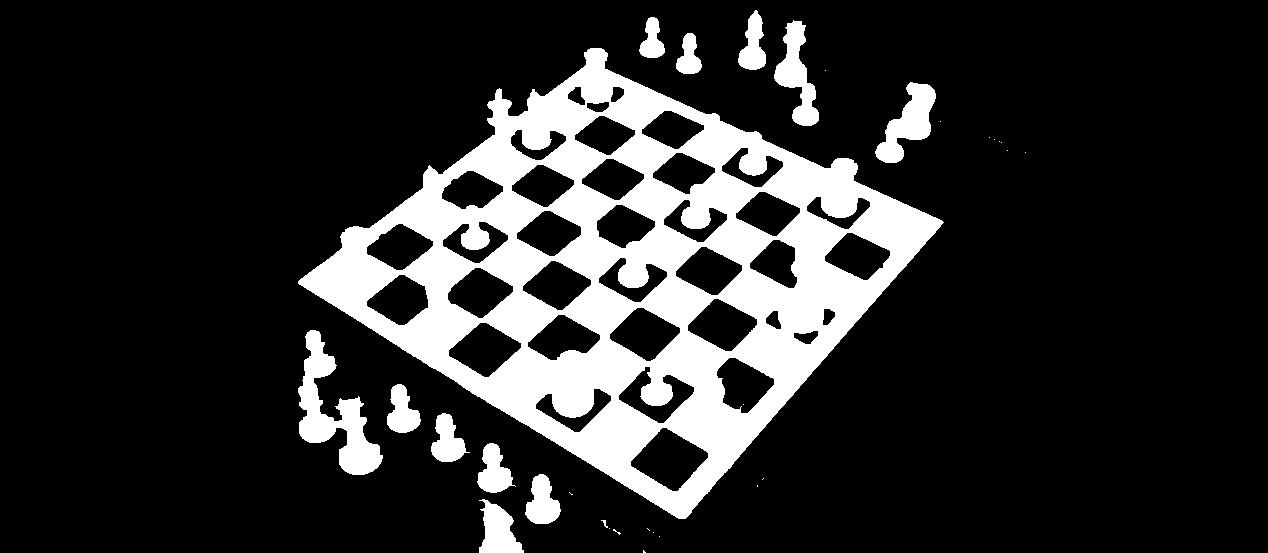
\includegraphics[width=4cm,height=2cm]{binary.jpg}
    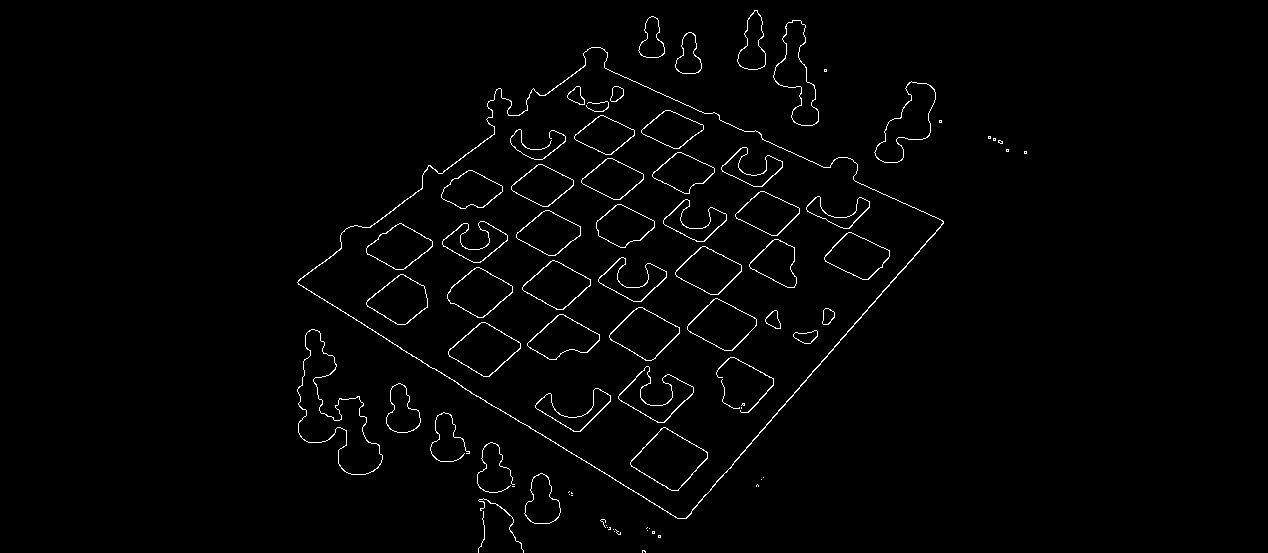
\includegraphics[width=4cm,height=2cm]{canny.jpg}\\ \\
    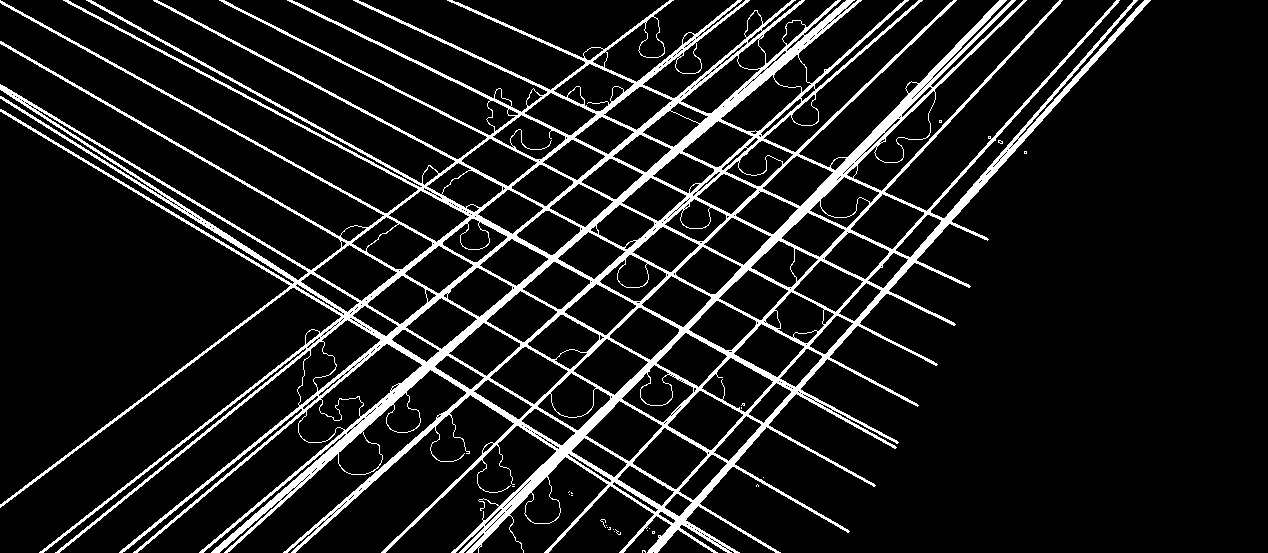
\includegraphics[width=4cm,height=2cm]{Hough.jpg}
    \caption{Binary image after Otsu's representation, Image after Canny, Image after Hough}
\end{figure}

\begin{figure}[bhp]
	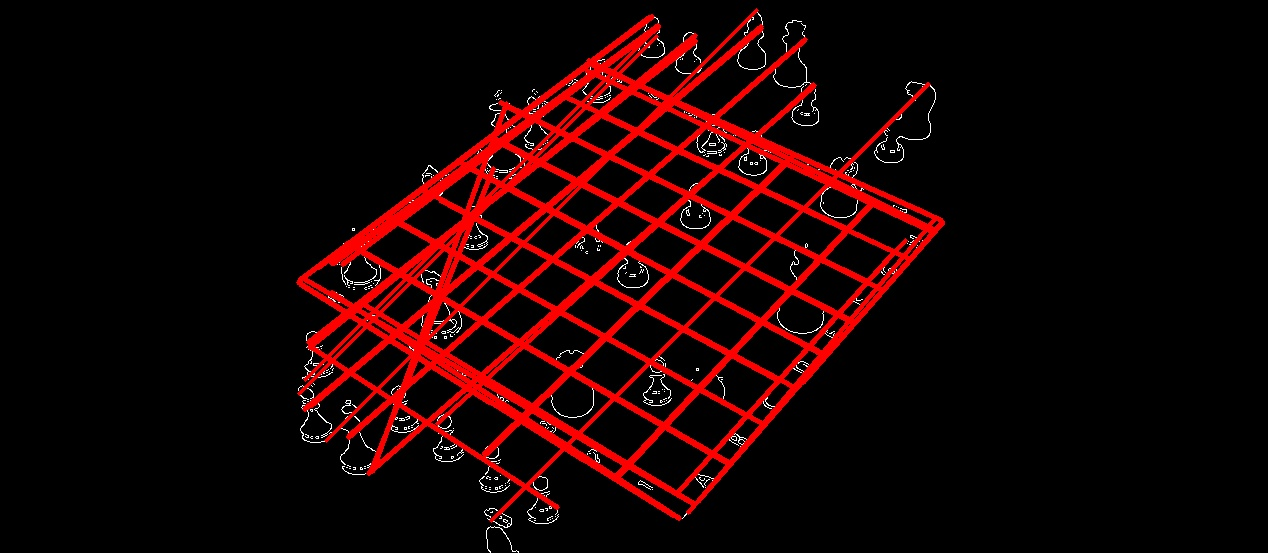
\includegraphics[width=4cm,height=2cm]{HoughLines.jpg}
	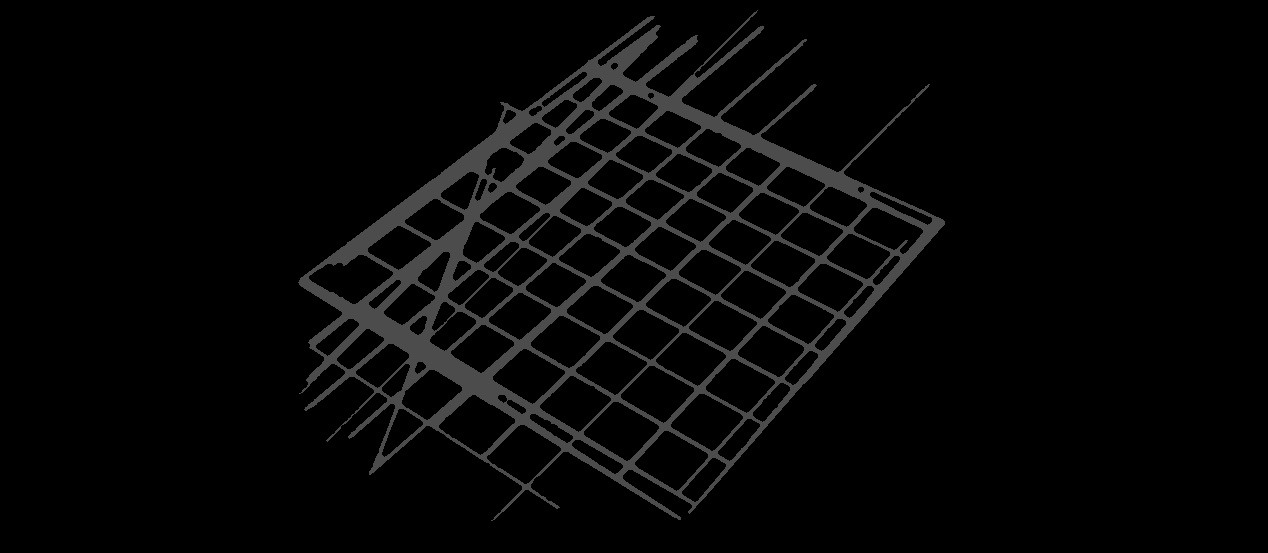
\includegraphics[width=4cm,height=2cm]{Result.jpg}\\
	\caption{C++ implementation - Hough Lines with chess pieces and result without chess pieces}
\end{figure}
We tried to implement the similar functionality using C++ with OpenCV package. We came to a phase wherein we could mask the chess pieces from the keyboard and erode the image to eliminate noises. But we struggled to continue with the piece detection phase and the results were not up to the mark. Fig 2 represents the results achieved using OpenCV implementation of C++. 

We also tried implementing the algorithm using Matlab, using which we found more success. We integrated the Computer Vision System Toolbox with Matlab[7] and tried to implement the algorithm. We could achieve the results up to a phase where we segmented the chess board and retained only the chess pawns. As you will see below, the results are much better with Matlab and the programming was also simple - 

\begin{figure}[bhp]
	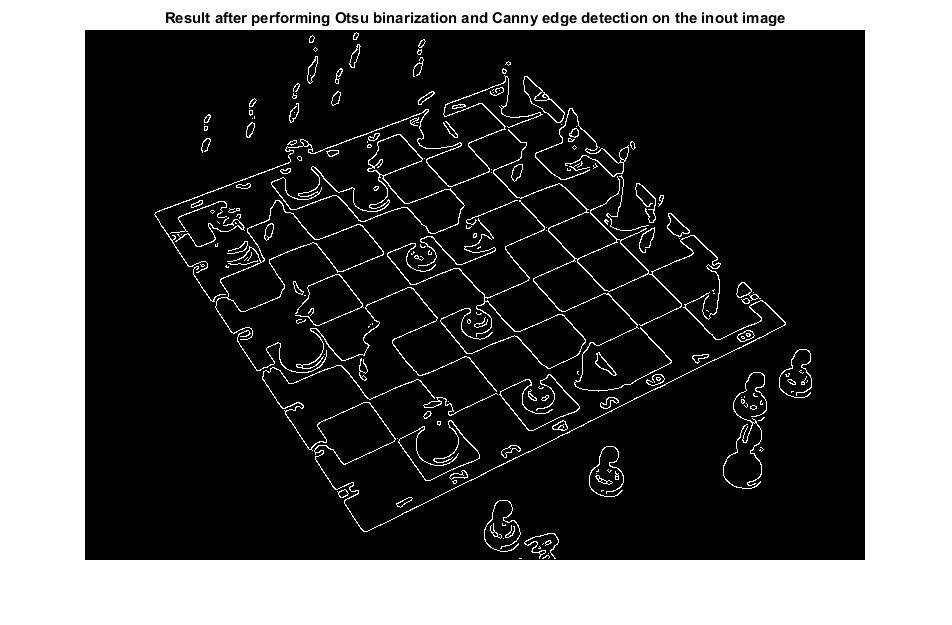
\includegraphics[width=4cm,height=2cm]{1.jpg}
	\includegraphics[width=4cm,height=2cm]{2.jpg}\\ \\
	\includegraphics[width=4cm,height=2cm]{3.jpg}
	\includegraphics[width=4cm,height=2cm]{4.jpg}\\ \\
	\includegraphics[width=4cm,height=2cm]{5.jpg}
	\includegraphics[width=4cm,height=2cm]{6.jpg}\\ \\
	\caption{Images after each step using Matlab implementation}
\end{figure}


\section{Improvements}
\subsection{Chess piece detection}
We had planned initially to extract each chess piece from the chessboard, orient it with respect to the training set and calculate the area score. But due to the challenges faced during implementations, we could not complete this task. 
\subsection{Orientation of the image}
This algorithm will work for viewing angles between 30 to 60 degrees and will fail for other orientations. We need to come up with a better solution to recognize the chess board for all viewing angles. 
\subsection{Correctness of the game}
For the detected pieces, we can check for correctness of the game by ensuring correct number of pawns are present on the board. For example, if there are 3 queens in the image, then the algorithm should give an invalid input message.
\subsection{Intelligence to the algorithm}
Once the pieces are recognized, intelligence can be added to predict the next best move of a particular piece. 

\section{Conclusion}
This paper presents an algorithm to recognize the chess board using image processing techniques such as Otsu's binarization, Canny's edge detection and Hough transform, extract the chess pieces out of the board and measure the accuracy of the detected pieces. Our implementation involves coding in C++, Python and Matlab, results of which are represented in section 3. 	

Due to the implementation challenges faced as described in section 3, we could not complete the piece detection phase, however, we were able to understand the idea behind detecting chess pieces and we are planning to finish what we started(build an AI for predicting the next best move) during our summer break.




% conference papers do not normally have an appendix
\section*{How to run the code}
1. For Python - ``python chess.py" \newline
2. For C++ - ``make main" and ``./main image" \newline
3. Matlab - Install matlab and integrate it with OpenCV using the reference[7]. Please note that Computer Vision System Toolbox must be installed while installing Matlab(it comes as a package). Install an appropriate c++ compiler (Visual studio 2012 preferred). Please refer to the documentation at[8]. Once the complete setup is done, run the file "Main.m" using Matlab tool. 

% use section* for acknowledgment
\section*{Acknowledgment}
We thank Dr. David Crandall for his support and guidance during the understanding and implementation of the project. We also want to thank the AIs for their continuous support. This course was really helpful in understanding the core concepts of vision and image processing techniques. 

% trigger a \newpage just before the given reference
% number - used to balance the columns on the last page
% adjust value as needed - may need to be readjusted if
% the document is modified later
%\IEEEtriggeratref{8}
% The "triggered" command can be changed if desired:
%\IEEEtriggercmd{\enlargethispage{-5in}}

% references section

% can use a bibliography generated by BibTeX as a .bbl file
% BibTeX documentation can be easily obtained at:
% http://mirror.ctan.org/biblio/bibtex/contrib/doc/
% The IEEEtran BibTeX style support page is at:
% http://www.michaelshell.org/tex/ieeetran/bibtex/
%\bibliographystyle{IEEEtran}
% argument is your BibTeX string definitions and bibliography database(s)
%\bibliography{IEEEabrv,../bib/paper}
%
% <OR> manually copy in the resultant .bbl file
% set second argument of \begin to the number of references
% (used to reserve space for the reference number labels box)
\begin{thebibliography}{1}

\bibitem{IEEEhowto:kopka}
Bhavani B.S, \emph{Chess State Detection}, Stanford University \newline

\bibitem{IEEEhowto:kopka}
Yangyang Yu, \emph{Chinese Chess State Recognition}, Standford University \newline

\bibitem{IEEEhowto:kopka}
Image Processing in OpenCV(Python), Image thresholding - \textit{http://docs.opencv.org/3.1.0/d7/d4d/tutorial\_py\_thresholding.html\#gsc.tab=0} \newline

\bibitem{IEEEhowto:kopka}
Image Processing in OpenCV(Python), Canny edge detection - \textit{http://docs.opencv.org/3.1.0/da/d22/tutorial\_py\_canny.html\#gsc.tab=0} \newline

\bibitem{IEEEhowto:kopka}
Image Processing in OpenCV(Python), Hough line transform - \textit{http://docs.opencv.org/3.0-beta/doc/py\_tutorials/py\_imgproc/py\_houghlines/py\_houghlines.html} \newline

\bibitem{IEEEhowto:kopka}
Koray, Can and Sumer,Emre , \emph{A Computer Vision System for Chess Game Tracking}, Baskent University \newline

\bibitem{IEEEhowto:kopka}
Matlab with OpenCV integration - \textit{http://www.mathworks.com/discovery/matlab-opencv.html?refresh=true} \newline

\bibitem{IEEEhowto:kopka}
C++ compiler setup for mex files in Matlab - \textit{http://www.mathworks.com/help/matlab/matlab\_external/choose-c-or-c-compilers.html} \newline

\bibitem{IEEEhowto:kopka}
Hinterstoisser, S. ; Lepetit, V. ; Ilic, S. ; Fua, P., “Dominant orientation templates for real-time detection of texture-less objects”, Computer Vision and Pattern Recognition (CVPR), 2010 IEEE Conference, pp 2257 – 2264, 13-18 June 2010 \newline

\bibitem{IEEEhowto:kopka}
Serge, Belongie; Jitendra, Malik; Jan, Puzicha, “Shape Matching and Object Recognition Using Shape Contexts”, IEEE Transaction on Pattern Analysis and Machine Intelligence, Vol. 24, April 2002

\end{thebibliography}




% that's all folks
\end{document}


